\documentclass{article}

% RTCA @ NeurIPS 2026 workshop submission (double-blind)
\usepackage[dblblindworkshop]{neurips_2026}
\workshoptitle{Real-Time Conversational Agents (RTCA)}

\usepackage[utf8]{inputenc} % allow utf-8 input
\usepackage[T1]{fontenc}    % use 8-bit T1 fonts
\usepackage{hyperref}       % hyperlinks
\usepackage{url}            % simple URL typesetting
\usepackage{booktabs}       % professional-quality tables
\usepackage{amsfonts}       % blackboard math symbols
\usepackage{nicefrac}       % compact symbols for 1/2, etc.
\usepackage{microtype}      % microtypography
\usepackage{xcolor}         % colors
\usepackage{graphicx}
\usepackage{amsmath}
\usepackage{amssymb}
\usepackage{tikz}
\usetikzlibrary{arrows.meta,positioning,shapes.geometric,fit,backgrounds}
% Local makecell replacement: provide \thead and \makecell without requiring makecell.sty
\newcommand{\thead}[1]{\begin{tabular}[c]{@{}c@{}}\bfseries\small #1\end{tabular}}
\newcommand{\makecell}[1]{\begin{tabular}[c]{@{}c@{}}#1\end{tabular}}

% Compact float spacing for the 4-page workshop limit
\setlength{\textfloatsep}{5pt plus 2pt minus 2pt}
\setlength{\floatsep}{5pt plus 2pt minus 2pt}
\setlength{\intextsep}{5pt plus 2pt minus 2pt}
\setlength{\abovecaptionskip}{3pt}
\setlength{\belowcaptionskip}{1pt}

\title{Dual-State KV Forking: Low-Overhead Semantic \\ Interruption for Full-Duplex LLM Agents}

\author{%
  Anonymous Author(s) \\
  Affiliation and Address omitted for double-blind review \\
}

\begin{document}

\maketitle

\begin{abstract}
Human conversation is full-duplex: listeners process speech continuously and interrupt mid-utterance to correct errors, volunteer answers, or take the floor. Multi-agent LLM systems remain half-duplex: a listener must wait for the speaker's entire turn, and input streaming---while it keeps the listener's cache warm---remains passive. We present the \textbf{Dual-State KV-Forking} architecture, which gives a streaming listener \emph{active} floor control. The listener maintains a progressively updated Base KV cache over the incoming stream; at each chunk boundary it forks this cache (0.01--0.06\,ms measured) into an ephemeral Assessor branch that appends a short decider prompt and emits a single logit-gated \texttt{STOP}/\texttt{CONTINUE} token, leaving the Base state intact. Each stream token is ingested exactly once, eliminating the $O(N^2 \cdot k)$ context re-prefill of a stateless independent decider while preserving a warm cache for instant response generation. Across three models on physical hardware, on FLEXI, Full-Duplex-Bench, and a 200-scenario progressive-clue floor-control task, our framework matches or exceeds independent-decider accuracy (up to 100\% on FDB), cuts total tokens processed per scenario by \textbf{78.6\%}, reduces Time-to-Halt by up to \textbf{49.1\%} under concurrent full-duplex streaming, and cuts no-interruption Time-to-First-Token by up to \textbf{65.0\%}.
\end{abstract}

\section{Introduction}
\label{sec:intro}

Human dialogue is fluid and full-duplex: listeners emit backchannels (``uh-huh'', ``right'') to signal comprehension without claiming the floor, and execute intentional barge-ins (``wait, stop'') when they detect an error, possess the answer, or must inject a constraint~\citep{sacks1974turntaking, yngve1970, skantze2021review}. LLM multi-agent systems~\citep{wu2023autogen, li2023camel}, however, are half-duplex: an agent waits passively for the speaker to complete its turn, forcing the speaker into an asymmetric dilemma---verbosity wastes tokens, latency, and context; brevity risks ambiguity---and leaving the listener powerless against hallucination, redundant tool calls, or obsolete instructions mid-stream. \emph{Input streaming}~\citep{xiao2023streamingllm, agrawal2023sarathi} partially addresses end-of-turn latency by prefilling tokens as they arrive, minimizing Time-to-First-Token (TTFT) once the speaker finishes---but it is passive; the listener still cannot seize the floor. What is missing is \textbf{semantic interruption assessment}: continuously classifying the incoming stream as \emph{intentional barge-in} (\texttt{STOP}) versus \emph{benign continuation} (\texttt{CONTINUE}).

The naive solution---invoking an independent LLM decider on every streaming chunk---introduces three bottlenecks. \textbf{(1) Quadratic re-prefill}: a stateless decider re-prefills the accumulated prefix of $m \cdot k$ tokens at every check $m$, a cumulative $\sum_{m=1}^{N} m k = O(N^2 \cdot k)$ prefill cost that dwarfs the dialogue itself in long interactions. \textbf{(2) Reasoning latency}: instruction-tuned deciders emit 15--35 chain-of-thought tokens before answering, adding seconds of delay to a millisecond-scale decision. \textbf{(3) Cold-start TTFT}: if no interruption fires, the decider's transient context is discarded and the listener must re-prefill the full $N \cdot k$ sequence before responding.

We introduce the \textbf{Dual-State KV-Forking} architecture (Figure~\ref{fig:dual_state_arch}). A \emph{Base state} ingests the stream once, chunk by chunk, into a persistent KV cache. At each chunk boundary, the cache is forked---via shallow tensor cloning, measured at 0.01--0.06\,ms---into an ephemeral \emph{Assessor state} that appends a short decider prompt and emits a single token constrained by logit gating to $\{\texttt{STOP}, \texttt{CONTINUE}\}$. The fork is discarded after the decision; the Base cache is never touched, so it remains warm for instant response generation if the speaker concludes naturally.

Our contributions are: \textbf{(i)} a dual-state execution scheme adding active, prompt-configurable interruption to streaming listeners with per-check prefill cost independent of history length, zero trained parameters, and no corruption of the response-generation state; \textbf{(ii)} a three-model physical-hardware study spanning interruption accuracy on FLEXI and Full-Duplex-Bench~\citep{lin2025fdbench} and end-to-end floor control on a 200-scenario progressive-clue task built on incremental QA~\citep{rodriguez2021quizbowl, wallace2019trick}; \textbf{(iii)} accuracy on par with (or better than) a reasoning independent decider at \textbf{78.6\%} fewer total tokens, up to \textbf{49.1\%} lower Time-to-Halt, and up to \textbf{65.0\%} lower no-op TTFT via the preserved streaming cache.

\begin{figure}[t]
\centering
\resizebox{0.72\textwidth}{!}{%
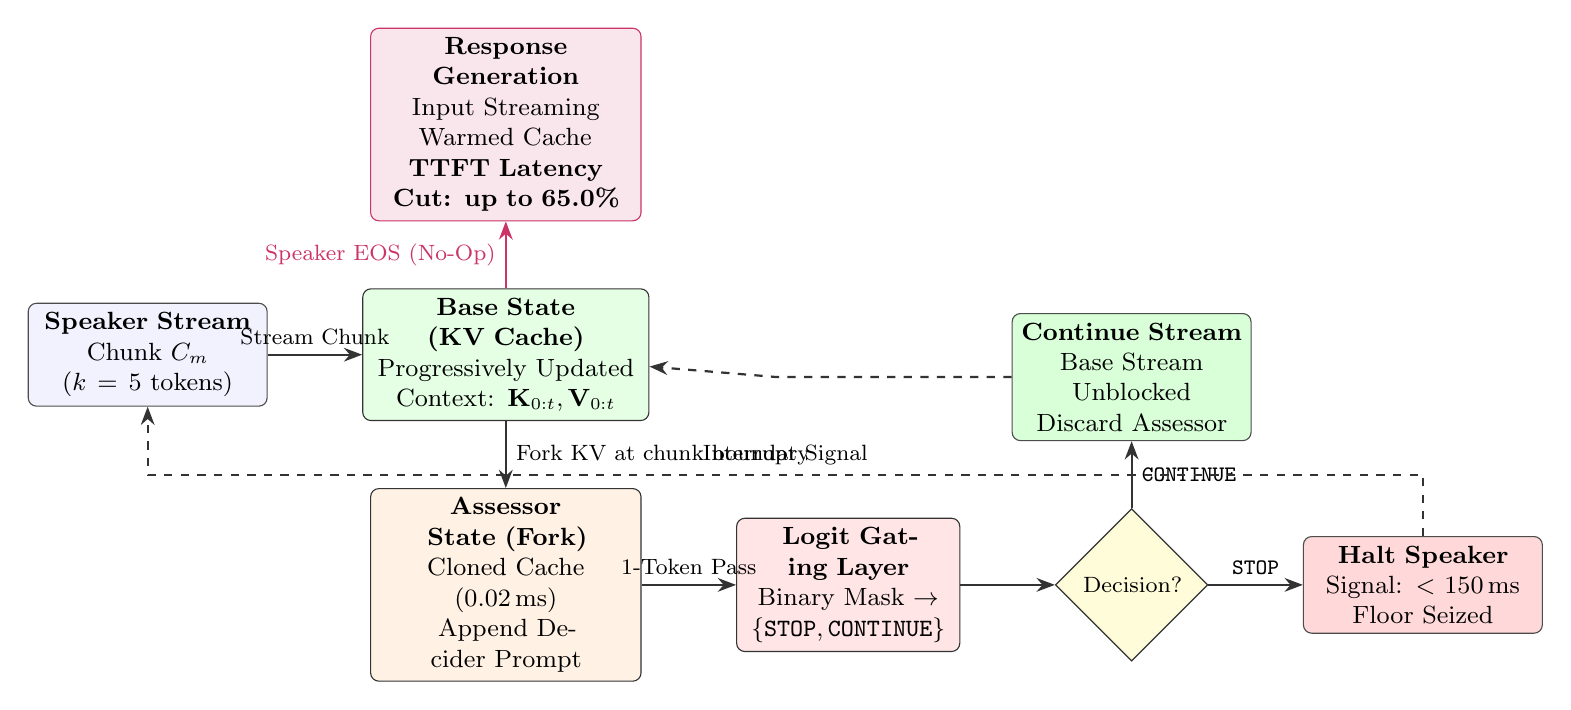
\begin{tikzpicture}[
    node distance=0.9cm and 1.2cm,
    box/.style={rectangle, draw=black!70, fill=blue!5, rounded corners=3pt, text width=2.8cm, align=center, minimum height=0.9cm, font=\small},
    statebox/.style={rectangle, draw=black!80, fill=green!10, rounded corners=3pt, text width=3.4cm, align=center, minimum height=1.0cm, font=\small},
    forkbox/.style={rectangle, draw=black!80, fill=orange!10, rounded corners=3pt, text width=3.2cm, align=center, minimum height=1.0cm, font=\small},
    gatebox/.style={rectangle, draw=black!80, fill=red!10, rounded corners=3pt, text width=2.6cm, align=center, minimum height=0.9cm, font=\small},
    decision/.style={diamond, draw=black!80, fill=yellow!15, text width=1.6cm, align=center, inner sep=1pt, font=\footnotesize},
    respbox/.style={rectangle, draw=purple!80, fill=purple!10, rounded corners=3pt, text width=3.2cm, align=center, minimum height=1.0cm, font=\small},
    arrow/.style={-{Stealth[scale=1.0]}, thick, draw=black!80}
]

% Nodes
\node[box] (speaker) {\textbf{Speaker Stream} \\ Chunk $C_m$ ($k=5$ tokens)};
\node[statebox, right=of speaker] (base) {\textbf{Base State (KV Cache)} \\ Progressively Updated \\ Context: $\mathbf{K}_{0:t}, \mathbf{V}_{0:t}$};
\node[forkbox, below=0.85cm of base] (assessor) {\textbf{Assessor State (Fork)} \\ Cloned Cache (0.02\,ms) \\ Append Decider Prompt};
\node[gatebox, right=of assessor] (gate) {\textbf{Logit Gating Layer} \\ Binary Mask $\to$ \\ $\{\texttt{STOP}, \texttt{CONTINUE}\}$};
\node[decision, right=of gate] (decision_node) {Decision?};
\node[box, above=0.85cm of decision_node, fill=green!15] (continue_node) {\textbf{Continue Stream} \\ Base Stream Unblocked \\ Discard Assessor};
\node[box, right=1.2cm of decision_node, fill=red!15] (halt_node) {\textbf{Halt Speaker} \\ Signal: $<150$\,ms \\ Floor Seized};
\node[respbox, above=0.85cm of base] (resp_node) {\textbf{Response Generation} \\ Input Streaming Warmed Cache \\ \textbf{TTFT Latency Cut: up to 65.0\%}};

% Edges
\draw[arrow] (speaker) -- node[above, font=\footnotesize] {Stream Chunk} (base);
\draw[arrow] (base) -- node[right, font=\footnotesize] {Fork KV at chunk boundary} (assessor);
\draw[arrow] (assessor) -- node[above, font=\footnotesize] {1-Token Pass} (gate);
\draw[arrow] (gate) -- (decision_node);
\draw[arrow] (decision_node) -- node[right, font=\footnotesize] {\texttt{CONTINUE}} (continue_node);
\draw[arrow] (decision_node) -- node[above, font=\footnotesize] {\texttt{STOP}} (halt_node);
\draw[arrow, dashed] (continue_node) -- ++(-4.5,0) -- (base);
\draw[arrow, dashed] (halt_node) |- ++(0,1.4) -| node[pos=0.25, above, font=\footnotesize] {Interrupt Signal} (speaker);
\draw[arrow, thick, color=purple!80] (base) -- node[left, font=\footnotesize] {Speaker EOS (No-Op)} (resp_node);

\end{tikzpicture}%
}
\caption{\textbf{Dual-State KV-Forking.} Speaker chunks update the Base cache ($O(k)$/chunk). At each boundary the cache is forked ($\le$0.06\,ms) into an Assessor emitting one gated \texttt{STOP}/\texttt{CONTINUE} token. \texttt{CONTINUE} discards the fork; \texttt{STOP} halts the speaker in sub-150\,ms; on natural completion the warm cache generates the response immediately.}
\label{fig:dual_state_arch}
\end{figure}

\section{Related Work}
\label{sec:related}

\textbf{Full-duplex spoken dialogue.} Turn-taking, overlap, and backchannels are foundational in conversation analysis~\citep{sacks1974turntaking, yngve1970} and long engineered into spoken dialogue systems~\citep{skantze2021review, lin2022duplex}. Neural full-duplex models jointly listen and speak---dGSLM~\citep{nguyen2023dgslm}, Moshi~\citep{defossez2024moshi}, Mini-Omni2~\citep{xie2024miniomni2}, duplex-tuned LLMs~\citep{zhang2024duplexmodels}---while Full-Duplex-Bench~\citep{lin2025fdbench, lin2025fdbenchv2} and SID-Bench~\citep{xia2026sidbench} standardize evaluation of pause handling, backchanneling, turn-taking, and semantic interruption detection. These works target the speech interface of a \emph{single} agent facing a human; we target the complementary problem of \emph{agent-to-agent} floor control in text-token streams with a frozen LLM listener.

\textbf{Streaming ingestion and KV reuse.} Chunked prefill~\citep{agrawal2023sarathi}, attention sinks~\citep{xiao2023streamingllm}, continuous batching~\citep{yu2022orca}, paged KV memory~\citep{kwon2023vllm}, radix-tree prefix sharing~\citep{zheng2023sglang}, prompt caching~\citep{gim2024promptcache}, and speculative decoding~\citep{leviathan2023speculative} all reuse or cheaply extend computed state to cut latency and memory. Our contribution is not a new cache mechanism but a \emph{dual-state execution pattern} over these primitives---a persistent streaming trunk plus ephemeral copy-on-write assessment branches---applied to real-time interruption; it maps natively onto RadixAttention/PagedAttention (Appendix~\ref{app:serving}).

\textbf{Multi-agent LLM systems and incremental QA.} Multi-agent frameworks such as AutoGen~\citep{wu2023autogen} and CAMEL~\citep{li2023camel} coordinate agents through strictly sequential message exchange. Incremental QA---Quizbowl~\citep{rodriguez2021quizbowl} and adversarially authored questions~\citep{wallace2019trick}---provides a natural testbed for \emph{when to buzz}, which we adapt as a full-duplex floor-control benchmark.

\section{The Dual-State KV-Forking Framework}
\label{sec:method}

The framework decomposes stream comprehension into two decoupled execution states (Figure~\ref{fig:dual_state_arch}).

\textbf{Base state: continuous streaming ingestion.} Let $S = (x_1, \dots, x_T)$ be the speaker's token sequence, arriving in chunks $C_m = (x_{(m-1)k+1}, \dots, x_{mk})$, $m \in \{1, \dots, M\}$. On receiving $C_m$, the Base state computes projections only for the new tokens ($\mathbf{K}_{\text{new}}^{(m)} = C_m \mathbf{W}_K$, $\mathbf{V}_{\text{new}}^{(m)} = C_m \mathbf{W}_V$), appends them to the cache, $\mathbf{K}_{\text{base}}^{(m)} = [ \mathbf{K}_{\text{base}}^{(m-1)} \| \mathbf{K}_{\text{new}}^{(m)} ]$ (analogously for $\mathbf{V}$), and attends $\mathbf{Q}_{\text{new}}^{(m)}$ causally over the accumulated cache. Past KV states persist, so each stream token is ingested exactly once: cumulative prefill cost is linear, $\mathcal{T}_{\text{base}} = \sum_{m=1}^{M} k = T$.

\textbf{Assessor state: low-overhead KV forking.} To evaluate an interruption at chunk $m$, the system forks the Base cache, $(\mathbf{K}, \mathbf{V})_{\text{assessor}}^{(m)} \leftarrow (\mathbf{K}, \mathbf{V})_{\text{base}}^{(m)}$, via pointer aliasing (measured as 0.01--0.06\,ms deep-clone overhead in our PyTorch validation prototype, and zero-copy in production engines; Appendix~\ref{app:serving}). The fork isolates the assessment: the decider prompt never contaminates the Base cache, which continues ingesting the live stream.

\textbf{Logit gating.} The Assessor appends a fixed decider prompt $\mathbf{P}_{\text{eval}}$ ($L_p = 10$ tokens) and executes a single forward pass, yielding logits $\mathbf{z}^{(m)}$ at the final position. Generation is constrained to the binary subspace $\{\text{id}(\texttt{STOP}), \text{id}(\texttt{CONTINUE})\}$ with decision $\hat{y}^{(m)} = \texttt{STOP} \iff z_{\texttt{STOP}} > z_{\texttt{CONTINUE}}$---the natural argmax boundary, requiring no threshold tuning. Because the policy lives entirely in $\mathbf{P}_{\text{eval}}$, interruption criteria are reconfigurable at runtime with zero retraining---unlike trained auxiliary probes (Appendix~\ref{app:probes}).

\textbf{No-op path.} If the speaker concludes without interruption, the warm Base cache turns response TTFT from an $O(L)$ cold prefill into a single-step decode. This gain is driven by input streaming itself; Dual-State's contribution is enabling concurrent mid-stream assessment \emph{without} evicting, corrupting, or duplicating that cache.

\section{Experiments}
\label{sec:exp}

\textbf{Setup.} All experiments run on physical hardware (NVIDIA RTX~4070~Ti, 4-bit precision) with Gemma~4~12B~\citep{gemmateam2026gemma4}, Llama~3.1~8B~\citep{grattafiori2024llama3}, and Qwen~3~4B~\citep{yang2025qwen3}. We compare four architectures: \textbf{(A) Independent Decider}, a stateless LLM called on every chunk with the full accumulated context, generating free-form reasoning (15--35 tokens) before deciding; \textbf{(B) Thought Bypass}, variant of A injecting closed-thought blocks to skip internal reasoning (Gemma only; Appendix~\ref{app:full_tables}); \textbf{(C) Independent + Logit Gating}, stateless full-context re-prefill with a 1-token gated decision, isolating the pure re-prefill penalty; \textbf{(D) Dual-State (ours)}, forked streaming cache with a 1-token gated decision.

\textbf{Benchmarks.} (i) \textbf{FLEXI}: 400 human dialogue transcripts (200 intentional barge-ins, 200 benign backchannels); (ii) \textbf{Full-Duplex-Bench (FDB)}~\citep{lin2025fdbench}: 400 dynamic multi-agent roleplay scenarios with semantic ground truth; (iii) \textbf{progressive-clue floor control} (Section~\ref{sec:handraiser}).

\subsection{Interruption Accuracy and Latency}
\label{sec:accuracy}

Table~\ref{tab:main_results} summarizes accuracy and latency (full per-model ablations, including thought bypass and confusion matrices, in Appendix~\ref{app:full_tables}).

\begin{table}[t]
\centering
\caption{\textbf{Interruption accuracy and physical latency.} Avg.\ latency is mean per-check decision latency on FDB; Time-to-Halt is measured on true positives. Full tables with confusion matrices and FLEXI latencies in Appendix~\ref{app:full_tables}.}
\label{tab:main_results}
\renewcommand{\arraystretch}{0.88}
\resizebox{\textwidth}{!}{%
\begin{tabular}{@{}llcccc@{}}
\toprule
\textbf{Model} & \textbf{Architecture} & \textbf{FLEXI Acc.} & \textbf{FDB Acc.} & \textbf{Avg.\ FDB Latency} & \textbf{Time-to-Halt (FDB TP)} \\ \midrule
\textbf{Gemma 4 12B} & Independent (reasoning) & \textbf{99.75\%} & 99.50\% & 2452.00\,ms & 1117.61\,ms \\
 & Independent + Logit Gating & 98.75\% & 90.75\% & 266.06\,ms & 268.46\,ms \\
 & \textbf{Dual-State (ours)} & 98.75\% & \textbf{100.00\%} & \textbf{90.26\,ms} & \textbf{180.53\,ms} \\ \midrule
\textbf{Llama 3.1 8B} & Independent (reasoning) & \textbf{93.50\%} & \textbf{97.00\%} & 361.96\,ms & 518.45\,ms \\
 & Independent + Logit Gating & 91.00\% & 95.00\% & 117.07\,ms & 117.67\,ms \\
 & \textbf{Dual-State (ours)} & 90.50\% & 94.25\% & \textbf{57.87\,ms} & \textbf{115.73\,ms} \\ \midrule
\textbf{Qwen 3 4B} & Independent (reasoning) & 97.50\% & \textbf{99.75\%} & 189.64\,ms & 191.19\,ms \\
 & Independent + Logit Gating & 98.75\% & \textbf{99.75\%} & 122.35\,ms & 122.63\,ms \\
 & \textbf{Dual-State (ours)} & \textbf{99.00\%} & 99.50\% & \textbf{42.42\,ms} & \textbf{85.70\,ms} \\ \bottomrule
\end{tabular}%
}
\end{table}

\textbf{Accuracy is preserved without reasoning tokens.} The reasoning independent decider is accurate (99.75\% FLEXI on Gemma) but unusable in real time: its average per-check latency on FDB reaches \textbf{2{,}452\,ms}. Gated 1-token decisions retain 90.5--100\% accuracy across all models, and Dual-State matches or exceeds the gated independent decider (100.0\% vs.\ 90.75\% FDB on Gemma).

\textbf{Time-to-Halt.} Measured from the arrival of the critical token to the halt command, Dual-State cuts Time-to-Halt from 518\,ms to \textbf{116\,ms} on Llama ($\sim$78\%), 1{,}118\,ms to \textbf{181\,ms} on Gemma, and 191\,ms to \textbf{86\,ms} on Qwen---28--30\% below even the 1-token gated independent decider on Qwen and Gemma, and matching the memory-bandwidth floor on Llama FDB (115.7\,ms vs 117.7\,ms), purely from eliminating re-prefill. This responsiveness--stability trade-off directly mirrors the Average Penalty Time (APT) objective of semantic interruption detection~\citep{xia2026sidbench}.

\textbf{No-op TTFT.} When the stream completes without interruption, the preserved cache turns response TTFT into a single decode step: at $L{=}1024$, TTFT drops by \textbf{65.0\%} on Llama (234.65\,ms $\to$ 82.18\,ms), \textbf{48.7\%} on Gemma, and \textbf{36.0\%} on Qwen (full sweep in Appendix~\ref{app:ttft}). Fork overhead never exceeds 0.06\,ms.

\subsection{Full-Duplex Floor Control: Progressive-Clue Benchmark}
\label{sec:handraiser}

To evaluate end-to-end floor control, we adapt incremental QA~\citep{rodriguez2021quizbowl} to a full-duplex protocol (\textsc{Handraiser}): a speaker streams progressively more specific clues about a target entity ($k{=}5$ token chunks, 75\,ms intervals); at each boundary the listener may buzz (\texttt{STOP}) and guess. Incorrect guesses incur a penalty but the stream resumes, permitting later buzzes. The 200 scenarios comprise 100 adversarial questions from \texttt{AdvQA}~\citep{wallace2019trick} and 100 from \texttt{protobowl-11-13}; a game score rewards early accurate floor-taking (protocol and scoring in Appendix~\ref{app:handraiser}).

\begin{table}[t]
\centering
\caption{\textbf{\textsc{Handraiser} continuous multi-attempt floor control (200 scenarios, $k{=}5$).} Context re-prefill is cumulative redundant prefix tokens across all attempts per scenario (single-pass baseline is 576.2 tok; Appendix~\ref{app:tokens}).}
\label{tab:handraiser_results}
\renewcommand{\arraystretch}{0.88}
\resizebox{\textwidth}{!}{%
\begin{tabular}{@{}llccccc@{}}
\toprule
\textbf{Model} & \textbf{Architecture} & \textbf{Resolution Acc.} & \textbf{Game Score ($S$)} & \textbf{Time-to-Halt (s)} & \textbf{Consensus Time (s)} & \textbf{Context Re-Prefill} \\ \midrule
\textbf{Gemma 4 12B} & Independent Decider & 49.0\% & 6.11 & 0.2437 & 6.6435 & 2661.4 tok \\
 & \textbf{Dual-State (ours)} & \textbf{51.5\%} & \textbf{6.50} (\textit{+6.4\%}) & \textbf{0.1492} (\textit{-38.8\%}) & \textbf{5.6832} (\textit{-14.5\%}) & \textbf{0.0 tok} (\textit{-100\%}) \\ \midrule
\textbf{Llama 3.1 8B} & Independent Decider & 51.5\% & 5.93 & 0.1085 & 2.5378 & 3186.5 tok \\
 & \textbf{Dual-State (ours)} & \textbf{54.0\%} & \textbf{6.59} (\textit{+11.1\%}) & \textbf{0.0552} (\textit{-49.1\%}) & \textbf{2.0532} (\textit{-19.1\%}) & \textbf{0.0 tok} (\textit{-100\%}) \\ \midrule
\textbf{Qwen 3 4B} & Independent Decider & 43.0\% & 4.92 & 0.0934 & \textbf{3.0786} & 3121.9 tok \\
 & \textbf{Dual-State (ours)} & \textbf{44.0\%} & \textbf{4.97} (\textit{+1.0\%}) & \textbf{0.0857} (\textit{-8.2\%}) & 4.0542 & \textbf{0.0 tok} (\textit{-100\%}) \\ \bottomrule
\end{tabular}%
}
\end{table}

\textbf{Results} (Table~\ref{tab:handraiser_results}). Under concurrent full-duplex streaming, Dual-State (i) eliminates redundant context re-prefill entirely (the stateless baseline wastes 2{,}661--3{,}187 cumulative prefix tokens per scenario); (ii) cuts Time-to-Halt by up to 49.1\%; (iii) accelerates consensus by up to 19.1\% on Llama (while on Qwen, earlier non-fatal buzzes permit additional clue intake, trading consensus duration for higher resolution accuracy); and (iv) attains strictly higher resolution accuracy and game scores across all three families. In total accounting (Appendix~\ref{app:tokens}), the stateless decider consumes 966.3 tokens per 63.4-token scenario ($+1424\%$ overage) versus \textbf{207.2} for Dual-State ($+227\%$)---a \textbf{78.6\%} net reduction. A chunk-stride sweep ($k \in \{2, 5, 10, 20, 50\}$) shows strides $k \in [5, 10]$ achieve an optimal responsiveness--compute Pareto frontier; trained linear/MLP probes are faster (0.08--0.10\,ms) but require task-specific retraining, whereas Dual-State is fully zero-shot (Appendix~\ref{app:probes}).

\section{Discussion, Limitations, and Conclusion}
\label{sec:discussion}

\textbf{Serving integration \& memory.} The fork is a copy-on-write leaf on the RadixAttention~\citep{zheng2023sglang} trunk, or block-table sharing in PagedAttention~\citep{kwon2023vllm}. Aliasing rather than duplicating the trunk cuts per-stream assessor KV overhead from 90.9\,MB to 0.88\,MB ($\sim$49.5\% at batch 64; Appendix~\ref{app:serving}).
\textbf{Limitations.} (i) Our baseline is \emph{stateless}, reflecting decider-as-a-service deployments; a stateful variant would avoid re-prefill at the cost of duplicated ingestion compute and KV memory. (ii) Each assessment attends over the full cached history. (iii) Multi-party arbitration, spoken full-duplex integration~\citep{defossez2024moshi}, and human perceptual studies remain open.
\textbf{Conclusion.} Dual-State KV-Forking turns a passive streaming listener into an active conversational participant: one persistent cache ingests the stream once; ephemeral forks decide when to take the floor---a reusable building block for real-time full-duplex agent systems.

\begin{thebibliography}{25}
\providecommand{\natexlab}[1]{#1}
\providecommand{\url}[1]{\texttt{#1}}
\expandafter\ifx\csname urlstyle\endcsname\relax
  \providecommand{\doi}[1]{doi: #1}\else
  \providecommand{\doi}{doi: \begingroup \urlstyle{rm}\Url}\fi

\bibitem[Agrawal et~al.(2024)Agrawal, Kedia, Panwar, Mohan, Kwatra, Gulavani, Tumanov, and Ramjee]{agrawal2023sarathi}
Amey Agrawal, Nitin Kedia, Ashish Panwar, Jayashree Mohan, Nipun Kwatra, Bhargav~S. Gulavani, Alexey Tumanov, and Ramachandran Ramjee.
\newblock Taming throughput-latency tradeoff in {LLM} inference with {Sarathi-Serve}.
\newblock In \emph{Proceedings of the 18th USENIX Symposium on Operating Systems Design and Implementation (OSDI '24)}, pages 1127--1143, 2024.

\bibitem[D{\'e}fossez et~al.(2024)D{\'e}fossez, Mazar{\'e}, Orsini, Royer, P{\'e}rez, J{\'e}gou, Grave, and Zeghidour]{defossez2024moshi}
Alexandre D{\'e}fossez, Laurent Mazar{\'e}, Manu Orsini, Am{\'e}lie Royer, Patrick P{\'e}rez, Herv{\'e} J{\'e}gou, Edouard Grave, and Neil Zeghidour.
\newblock {Moshi}: a speech-text foundation model for real-time dialogue.
\newblock \emph{arXiv preprint arXiv:2410.00037}, 2024.

\bibitem[{Gemma Team}(2026)]{gemmateam2026gemma4}
{Gemma Team}.
\newblock {Gemma} 4 technical report.
\newblock \emph{arXiv preprint arXiv:2607.02770}, 2026.

\bibitem[Gim et~al.(2024)Gim, Chen, Lee, Sarda, Khandelwal, and Zhong]{gim2024promptcache}
In~Gim, Guojun Chen, Seung-seob Lee, Nikhil Sarda, Anurag Khandelwal, and Lin Zhong.
\newblock {Prompt Cache}: Modular attention reuse for low-latency inference.
\newblock In \emph{Proceedings of Machine Learning and Systems (MLSys)}, volume~6, pages 341--353, 2024.

\bibitem[Grattafiori et~al.(2024)Grattafiori et~al.]{grattafiori2024llama3}
Aaron Grattafiori et~al.
\newblock The {Llama} 3 herd of models.
\newblock \emph{arXiv preprint arXiv:2407.21783}, 2024.

\bibitem[Kwon et~al.(2023)Kwon, Li, Zhuang, Sheng, Zheng, Yu, Gonzalez, Zhang, and Stoica]{kwon2023vllm}
Woosuk Kwon, Zhuohan Li, Siyuan Zhuang, Ying Sheng, Lianmin Zheng, Cody~Hao Yu, Joseph~E. Gonzalez, Hao Zhang, and Ion Stoica.
\newblock Efficient memory management for large language model serving with {PagedAttention}.
\newblock In \emph{Proceedings of the 29th ACM Symposium on Operating Systems Principles (SOSP '23)}, pages 611--626, 2023.

\bibitem[Leviathan et~al.(2023)Leviathan, Kalman, and Matias]{leviathan2023speculative}
Yaniv Leviathan, Matan Kalman, and Yossi Matias.
\newblock Fast inference from transformers via speculative decoding.
\newblock In \emph{Proceedings of the 40th International Conference on Machine Learning (ICML '23)}, volume 202 of \emph{PMLR}, pages 19274--19286, 2023.

\bibitem[Li et~al.(2023)Li, Hammoud, Itani, Khizbullin, and Ghanem]{li2023camel}
Guohao Li, Hasan~Abed Al~Kader Hammoud, Hani Itani, Dmitrii Khizbullin, and Bernard Ghanem.
\newblock {CAMEL}: Communicative agents for ``mind'' exploration of large language model society.
\newblock In \emph{Advances in Neural Information Processing Systems (NeurIPS)}, volume~36, pages 51991--52008, 2023.

\bibitem[Lin et~al.(2022)Lin, Wu, Huang, Si, Sun, and Li]{lin2022duplex}
Ting-En Lin, Yuchuan Wu, Fei Huang, Luo Si, Jian Sun, and Yongbin Li.
\newblock Duplex conversation: Towards human-like interaction in spoken dialogue systems.
\newblock In \emph{Proceedings of the 28th ACM SIGKDD Conference on Knowledge Discovery and Data Mining (KDD '22)}, pages 3438--3447, 2022.

\bibitem[Lin et~al.(2025{\natexlab{a}})Lin, Lian, Li, Wang, Anumanchipalli, Liu, and Lee]{lin2025fdbench}
Guan-Ting Lin, Jiachen Lian, Tingle Li, Qirui Wang, Gopala Anumanchipalli, Alexander~H. Liu, and Hung-yi Lee.
\newblock {Full-Duplex-Bench}: A benchmark to evaluate full-duplex spoken dialogue models on turn-taking capabilities.
\newblock In \emph{Proc.\ IEEE ASRU}, 2025{\natexlab{a}}. arXiv:2503.04721.

\bibitem[Lin et~al.(2025{\natexlab{b}})Lin, Lian, Li, Wang, Liu, and Lee]{lin2025fdbenchv2}
Guan-Ting Lin, Jiachen Lian, Tingle Li, Qirui Wang, Alexander~H. Liu, and Hung-yi Lee.
\newblock {Full-Duplex-Bench-v2}: A multi-turn evaluation framework for duplex dialogue systems with an automated examiner.
\newblock \emph{arXiv preprint arXiv:2507.03157}, 2025{\natexlab{b}}.

\bibitem[Nguyen et~al.(2023)Nguyen, Kharitonov, Copet, Adi, Hsu, Elkahky, Tomasello, Algayres, Sagot, Mohamed, and Dupoux]{nguyen2023dgslm}
Tu~Anh Nguyen, Eugene Kharitonov, Jade Copet, Yossi Adi, Wei-Ning Hsu, Ali Elkahky, Paden Tomasello, Robin Algayres, Beno{\^\i}t Sagot, Abdelrahman Mohamed, and Emmanuel Dupoux.
\newblock Generative spoken dialogue language modeling.
\newblock \emph{Transactions of the Association for Computational Linguistics}, 11:\penalty0 250--266, 2023.

\bibitem[Rodriguez et~al.(2019)Rodriguez, Feng, Iyyer, He, and Boyd-Graber]{rodriguez2021quizbowl}
Pedro Rodriguez, Shi Feng, Mohit Iyyer, He~He, and Jordan Boyd-Graber.
\newblock Quizbowl: The case for incremental question answering.
\newblock \emph{arXiv preprint arXiv:1904.04792}, 2019.

\bibitem[Sacks et~al.(1974)Sacks, Schegloff, and Jefferson]{sacks1974turntaking}
Harvey Sacks, Emanuel~A. Schegloff, and Gail Jefferson.
\newblock A simplest systematics for the organization of turn-taking for conversation.
\newblock \emph{Language}, 50\penalty0 (4):\penalty0 696--735, 1974.

\bibitem[Skantze(2021)]{skantze2021review}
Gabriel Skantze.
\newblock Turn-taking in conversational systems and human-robot interaction: A review.
\newblock \emph{Computer Speech \& Language}, 67:\penalty0 101178, 2021.

\bibitem[Wallace et~al.(2019)Wallace, Rodriguez, Feng, Yamada, and Boyd-Graber]{wallace2019trick}
Eric Wallace, Pedro Rodriguez, Shi Feng, Ikuya Yamada, and Jordan Boyd-Graber.
\newblock Trick me if you can: Human-in-the-loop generation of adversarial examples for question answering.
\newblock \emph{Transactions of the Association for Computational Linguistics}, 7:\penalty0 387--401, 2019.

\bibitem[Wu et~al.(2023)Wu, Bansal, Zhang, Wu, Li, Zhu, Jiang, Zhang, Zhang, Liu, Awadallah, White, Burger, and Wang]{wu2023autogen}
Qingyun Wu, Gagan Bansal, Jieyu Zhang, Yiran Wu, Beibin Li, Erkang Zhu, Li~Jiang, Xiaoyun Zhang, Shaokun Zhang, Jiale Liu, Ahmed~Hassan Awadallah, Ryen~W. White, Doug Burger, and Chi Wang.
\newblock {Auto{G}en}: Enabling next-gen {LLM} applications via multi-agent conversation.
\newblock \emph{arXiv preprint arXiv:2308.08155}, 2023.

\bibitem[Xia et~al.(2026)Xia, Mu, Shi, Xu, and Xie]{xia2026sidbench}
Kangxiang Xia, Bingshen Mu, Xian Shi, Jin Xu, and Lei Xie.
\newblock Semantic-aware interruption detection in spoken dialogue systems: Benchmark, metric, and model.
\newblock \emph{arXiv preprint arXiv:2603.24144}, 2026.

\bibitem[Xiao et~al.(2024)Xiao, Tian, Chen, Han, and Lewis]{xiao2023streamingllm}
Guangxuan Xiao, Yuandong Tian, Beidi Chen, Song Han, and Mike Lewis.
\newblock Efficient streaming language models with attention sinks.
\newblock In \emph{International Conference on Learning Representations (ICLR)}, 2024.

\bibitem[Xie and Wu(2024)]{xie2024miniomni2}
Zhifei Xie and Changqiao Wu.
\newblock {Mini-Omni2}: Towards open-source {GPT-4o} with vision, speech and duplex capabilities.
\newblock \emph{arXiv preprint arXiv:2410.11190}, 2024.

\bibitem[Yang et~al.(2025)Yang et~al.]{yang2025qwen3}
An~Yang et~al.
\newblock {Qwen3} technical report.
\newblock \emph{arXiv preprint arXiv:2505.09388}, 2025.

\bibitem[Yngve(1970)]{yngve1970}
Victor~H. Yngve.
\newblock On getting a word in edgewise.
\newblock In \emph{Papers from the Sixth Regional Meeting of the Chicago Linguistic Society}, pages 567--578, 1970.

\bibitem[Yu et~al.(2022)Yu, Jeong, Kim, Kim, and Chun]{yu2022orca}
Gyeong-In Yu, Joo~Seong Jeong, Geon-Woo Kim, Soojeong Kim, and Byung-Gon Chun.
\newblock {Orca}: A distributed serving system for transformer-based generative models.
\newblock In \emph{Proceedings of the 16th USENIX Symposium on Operating Systems Design and Implementation (OSDI '22)}, pages 521--538, 2022.

\bibitem[Zhang et~al.(2024)Zhang, Chen, Hu, Han, Xu, Xu, Zhao, Sun, and Liu]{zhang2024duplexmodels}
Xinrong Zhang, Yingfa Chen, Shengding Hu, Xu~Han, Zihang Xu, Yuanwei Xu, Weilin Zhao, Maosong Sun, and Zhiyuan Liu.
\newblock Beyond the turn-based game: Enabling real-time conversations with duplex models.
\newblock In \emph{Proceedings of the 2024 Conference on Empirical Methods in Natural Language Processing (EMNLP '24)}, pages 11543--11557, 2024.

\bibitem[Zheng et~al.(2024)Zheng, Yin, Xie, Sun, Huang, Yu, Cao, Kozyrakis, Stoica, Gonzalez, Barrett, and Sheng]{zheng2023sglang}
Lianmin Zheng, Liangsheng Yin, Zhiqiang Xie, Chuyue Sun, Jeff Huang, Cody~Hao Yu, Shiyi Cao, Christos Kozyrakis, Ion Stoica, Joseph~E. Gonzalez, Clark Barrett, and Ying Sheng.
\newblock {SGLang}: Efficient execution of structured language model programs.
\newblock In \emph{Advances in Neural Information Processing Systems (NeurIPS)}, volume~37, 2024.

\end{thebibliography}

\appendix

\section{Full Per-Model Ablation Tables}
\label{app:full_tables}

Tables~\ref{tab:gemma_ablation}--\ref{tab:qwen_ablation} report the complete architecture ablations per model, including confusion matrices (TP/TN/FP/FN over 200 positive and 200 negative examples per benchmark), FLEXI latencies, and---for Gemma---the thought-bypass variant, in which synthetic closed-thought blocks (\texttt{<|channel>thought\textbackslash n<channel|>}) are injected to force the model to skip internal reasoning. Thought bypass reduces latency relative to free-form reasoning but remains an order of magnitude slower than logit-gated decisions and is only applicable to models with explicit thought tags.

\begin{table}[h]
\centering
\caption{\textbf{Architecture ablation: Gemma 4 12B Instruct.} TP/TN/FP/FN reported below each accuracy. Latencies in ms; \emph{Blended} averages over interruption and no-op decisions.}
\label{tab:gemma_ablation}
\renewcommand{\arraystretch}{1.15}
\resizebox{\columnwidth}{!}{%
\begin{tabular}{@{}lcccc@{}}
\toprule
\thead{Metric} & \thead{Independent \\ (Baseline)} & \thead{Independent \\ (Thought Bypass)} & \thead{Independent \\ (Logit Gating)} & \thead{Dual-State \\ (Proposed)} \\ \midrule
\textbf{FLEXI Accuracy} & \makecell{\textbf{99.75\%} \\ \scriptsize TP\,200/TN\,199/FP\,1/FN\,0} & \makecell{\textbf{99.75\%} \\ \scriptsize TP\,200/TN\,199/FP\,1/FN\,0} & \makecell{98.75\% \\ \scriptsize TP\,200/TN\,195/FP\,5/FN\,0} & \makecell{98.75\% \\ \scriptsize TP\,200/TN\,195/FP\,5/FN\,0} \\
\textbf{FDB Accuracy} & \makecell{99.50\% \\ \scriptsize TP\,198/TN\,200/FP\,0/FN\,2} & \makecell{\textbf{100.00\%} \\ \scriptsize TP\,200/TN\,200/FP\,0/FN\,0} & \makecell{90.75\% \\ \scriptsize TP\,200/TN\,163/FP\,37/FN\,0} & \makecell{\textbf{100.00\%} \\ \scriptsize TP\,200/TN\,200/FP\,0/FN\,0} \\ \midrule
Avg.\ FLEXI decision latency (ms) & 1063.27 & 823.35 & 260.77 & \textbf{95.23} \\
Avg.\ FDB decision latency (ms) & 2452.00 & 1047.49 & 266.06 & \textbf{90.26} \\ \midrule
Time-to-Halt (FLEXI TP, ms) & 1131.24 & 759.33 & 265.01 & \textbf{190.46} \\
Time-to-Halt (FDB TP, ms) & 1117.61 & 746.42 & 268.46 & \textbf{180.53} \\ \bottomrule
\end{tabular}%
}
\end{table}

\begin{table}[h]
\centering
\caption{\textbf{Architecture ablation: Llama 3.1 8B Instruct.}}
\label{tab:llama_ablation}
\renewcommand{\arraystretch}{1.15}
\resizebox{\columnwidth}{!}{%
\begin{tabular}{@{}lccc@{}}
\toprule
\thead{Metric} & \thead{Independent \\ (Baseline)} & \thead{Independent \\ (Logit Gating)} & \thead{Dual-State \\ (Proposed)} \\ \midrule
\textbf{FLEXI Accuracy} & \makecell{\textbf{93.50\%} \\ \scriptsize TP\,177/TN\,197/FP\,3/FN\,23} & \makecell{91.00\% \\ \scriptsize TP\,166/TN\,198/FP\,2/FN\,34} & \makecell{90.50\% \\ \scriptsize TP\,162/TN\,200/FP\,0/FN\,38} \\
\textbf{FDB Accuracy} & \makecell{\textbf{97.00\%} \\ \scriptsize TP\,188/TN\,200/FP\,0/FN\,12} & \makecell{95.00\% \\ \scriptsize TP\,180/TN\,200/FP\,0/FN\,20} & \makecell{94.25\% \\ \scriptsize TP\,177/TN\,200/FP\,0/FN\,23} \\ \midrule
Avg.\ FLEXI decision latency (ms) & 384.77 & 117.60 & \textbf{39.46} \\
Avg.\ FDB decision latency (ms) & 361.96 & 117.07 & \textbf{57.87} \\ \midrule
Time-to-Halt (FLEXI TP, ms) & 555.19 & 119.79 & \textbf{78.91} \\
Time-to-Halt (FDB TP, ms) & 518.45 & 117.67 & \textbf{115.73} \\ \bottomrule
\end{tabular}%
}
\end{table}

\begin{table}[h]
\centering
\caption{\textbf{Architecture ablation: Qwen 3 4B Instruct} (4-bit quantization).}
\label{tab:qwen_ablation}
\renewcommand{\arraystretch}{1.15}
\resizebox{\columnwidth}{!}{%
\begin{tabular}{@{}lccc@{}}
\toprule
\thead{Metric} & \thead{Independent \\ (Baseline)} & \thead{Independent \\ (Logit Gating)} & \thead{Dual-State \\ (Proposed)} \\ \midrule
\textbf{FLEXI Accuracy} & \makecell{97.50\% \\ \scriptsize TP\,198/TN\,192/FP\,8/FN\,2} & \makecell{98.75\% \\ \scriptsize TP\,198/TN\,197/FP\,3/FN\,2} & \makecell{\textbf{99.00\%} \\ \scriptsize TP\,198/TN\,198/FP\,2/FN\,2} \\
\textbf{FDB Accuracy} & \makecell{\textbf{99.75\%} \\ \scriptsize TP\,199/TN\,200/FP\,0/FN\,1} & \makecell{\textbf{99.75\%} \\ \scriptsize TP\,199/TN\,200/FP\,0/FN\,1} & \makecell{99.50\% \\ \scriptsize TP\,198/TN\,200/FP\,0/FN\,2} \\ \midrule
Avg.\ FLEXI decision latency (ms) & 221.54 & 124.52 & \textbf{43.82} \\
Avg.\ FDB decision latency (ms) & 189.64 & 122.35 & \textbf{42.42} \\ \midrule
Time-to-Halt (FLEXI TP, ms) & 261.13 & 123.57 & \textbf{88.52} \\
Time-to-Halt (FDB TP, ms) & 191.19 & 122.63 & \textbf{85.70} \\ \bottomrule
\end{tabular}%
}
\end{table}

\section{No-Op TTFT Benchmark Across Context Lengths}
\label{app:ttft}

When an incoming utterance concludes without interruption (no-op), the listener must generate its first response token. We benchmark physical TTFT on NVIDIA RTX~4070~Ti in 4-bit precision across context lengths $L \in [64, 1024]$, comparing: \textbf{Baseline (cold prefill)}, in which the listener maintains no streaming cache and must prefill all $L$ context tokens before emitting the first token; and \textbf{Dual-State / input streaming (warmed)}, in which the Base cache was populated chunk-by-chunk during streaming and TTFT is a single-token decode. TTFT here measures exclusively local GPU latency ($T_{\text{prefill}} + T_{\text{decode},1}$), excluding network and API queuing overhead; full responses require subsequent autoregressive generation ($N_{\text{tokens}} \times 15$--$25$\,ms). Results are averaged over 3 independent runs per configuration. The primary physical driver of the gain is input streaming itself; Dual-State's contribution is enabling concurrent mid-stream interruption assessment without corrupting or evicting this cache.

\begin{table}[h]
\centering
\caption{\textbf{Physical no-op TTFT across context lengths} (RTX 4070 Ti, 4-bit, 3 runs).}
\label{tab:ttft_benchmark}
\vspace{0.2cm}
\resizebox{\textwidth}{!}{%
\begin{tabular}{@{}llccccc@{}}
\toprule
\textbf{Model} & \textbf{Architecture} & \textbf{$L=64$} & \textbf{$L=128$} & \textbf{$L=256$} & \textbf{$L=512$} & \textbf{$L=1024$} \\ \midrule
\textbf{Qwen 3 4B} & Baseline Cold TTFT & 85.00\,ms & 115.08\,ms & 100.26\,ms & 110.03\,ms & 136.47\,ms \\
 & \textbf{Dual-State Warmed TTFT} & \textbf{76.87\,ms} & \textbf{84.95\,ms} & \textbf{72.15\,ms} & \textbf{65.34\,ms} & \textbf{87.28\,ms} \\
 & \textit{Latency Reduction} & \textit{-9.6\%} & \textit{-26.2\%} & \textit{-28.0\%} & \textit{-40.6\%} & \textbf{-36.0\%} \\
 & Measured KV Fork Overhead & 0.01\,ms & 0.03\,ms & 0.02\,ms & 0.03\,ms & 0.03\,ms \\ \midrule
\textbf{Llama 3.1 8B} & Baseline Cold TTFT & 70.49\,ms & 74.75\,ms & 88.81\,ms & 141.36\,ms & 234.65\,ms \\
 & \textbf{Dual-State Warmed TTFT} & \textbf{56.12\,ms} & \textbf{60.16\,ms} & \textbf{40.81\,ms} & \textbf{69.14\,ms} & \textbf{82.18\,ms} \\
 & \textit{Latency Reduction} & \textit{-20.4\%} & \textit{-19.5\%} & \textit{-54.0\%} & \textit{-51.1\%} & \textbf{-65.0\%} \\
 & Measured KV Fork Overhead & 0.03\,ms & 0.02\,ms & 0.02\,ms & 0.03\,ms & 0.02\,ms \\ \midrule
\textbf{Gemma 4 12B} & Baseline Cold TTFT & 266.93\,ms & 242.29\,ms & 243.46\,ms & 280.28\,ms & 447.30\,ms \\
 & \textbf{Dual-State Warmed TTFT} & \textbf{228.38\,ms} & \textbf{237.09\,ms} & \textbf{162.73\,ms} & \textbf{229.26\,ms} & \textbf{229.46\,ms} \\
 & \textit{Latency Reduction} & \textit{-14.4\%} & \textit{-2.1\%} & \textit{-33.2\%} & \textit{-18.2\%} & \textbf{-48.7\%} \\
 & Measured KV Fork Overhead & 0.06\,ms & 0.05\,ms & 0.05\,ms & 0.05\,ms & 0.05\,ms \\ \bottomrule
\end{tabular}%
}
\end{table}

\section{\textsc{Handraiser} Protocol Details and Scoring}
\label{app:handraiser}

\textbf{Dataset.} A curated, balanced benchmark of 200 progressive-clue scenarios sampled from official repositories: exactly 100 adversarial human-crafted trivia questions from \texttt{qanta-challenge/AdvQA} (of 182 available) and 100 progressive-clue questions from \texttt{mgor/protobowl-11-13} (of 3{,}042 available). Average clue length is 63.4 tokens.

\textbf{Streaming turn-taking.} The speaker streams clues in discrete increments of $k=5$ tokens at 75\,ms intervals. Clues begin obscure and become progressively more specific.

\textbf{Continuous multi-attempt floor control.} At each chunk boundary, the listener evaluates whether to interrupt (\texttt{STOP}) or keep listening (\texttt{CONTINUE}). On interruption, it emits a concise entity guess. A correct guess solves and concludes the scenario. An incorrect guess incurs a penalty ($-\beta$) but \emph{the speaker resumes streaming remaining clues}, allowing the listener to buzz again as more discriminating information arrives. If all chunks conclude without a correct mid-stream buzz, the listener makes one final attempt on the complete clue.

\textbf{Scoring.} The game score rewards early, accurate floor-taking while penalizing hallucinated premature interruptions:
\begin{equation}
S_i = \mathbb{I}(\text{Solved}_i) \cdot \left[ B + \alpha \cdot \left(\frac{L_{\text{stream}, i} - L_{\text{solve}, i}}{L_{\text{stream}, i}}\right) \right] - \sum_{j=1}^{N_{\text{wrong}, i}} \beta
\label{eq:game_score}
\end{equation}
where $B = 10$ base points, $\alpha = 10$ maximum speed bonus, $\beta = 0.25$ penalty per incorrect buzz, and $L_{\text{solve}}$ is the token position at which the entity was correctly named.

\textbf{Metric disambiguation.} Scenario Resolution Accuracy in Table~\ref{tab:handraiser_results} measures end-to-end task completion on adversarial progressive trivia under multi-attempt dynamics, and should not be conflated with binary interruption precision: on FLEXI/FDB, Dual-State attains 97.25--100\% precision in classifying intentional barge-ins, while resolution accuracy (44.0--54.0\%) reflects the collaborative problem-solving capability of the listener on adversarially authored questions~\citep{wallace2019trick}, with Dual-State consistently outperforming the independent baseline by $+1.0$ to $+2.5$ points.

\section{Operational Token Accounting}
\label{app:tokens}

Table~\ref{tab:token_accounting} reports the complete token expenditure per scenario across the \textsc{Handraiser} benchmark (stream length 63.4 tokens, 13.1 chunks of $k=5$). The stateless independent decider must re-evaluate the accumulating context ($576.2$ tokens per single pass, escalating beyond $3{,}000$ tokens in multi-attempt games) plus its instruction prompt ($130.7$ tokens across 13.1 checks) and reasoning output (196.0 tokens), consuming \textbf{966.3 total tokens} per scenario ($+1424\%$ overage relative to the 63.4-token stream). Dual-State consumes \textbf{207.2 tokens} (63.4 stream + 130.7 assessor prompts + 13.1 gated decision tokens): a \textbf{78.6\%} net reduction, cutting overage to $+227\%$ ($-84.1\%$). Across 200 scenarios, the stateless baseline wastes over 600K prefill tokens on context re-ingestion alone.

\begin{table}[h]
\centering
\caption{\textbf{Token accounting breakdown per scenario (\textsc{Handraiser}, 200 scenarios).}}
\label{tab:token_accounting}
\vspace{0.2cm}
\resizebox{\columnwidth}{!}{%
\begin{tabular}{@{}lccc@{}}
\toprule
\textbf{Component} & \textbf{Independent Baseline} & \textbf{Dual-State (Proposed)} & \textbf{Net Reduction} \\ \midrule
Base Stream Ingestion & 63.4 tokens & 63.4 tokens & 0.0\% \\
Redundant Context Re-Prefill & 576.2 tokens & \textbf{0.0 tokens} & \textbf{-100.0\%} \\
Decider / Assessor Prompt Tokens ($L_p = 10$) & 130.7 tokens & 130.7 tokens & 0.0\% \\
Decider / Output Tokens & 196.0 tokens (Reasoning) & \textbf{13.1 tokens} (1-Token Gated) & \textbf{-93.3\%} \\ \midrule
\textbf{Total Tokens Processed} & \textbf{966.3 tokens} & \textbf{207.2 tokens} & \textbf{-78.6\%} \\
\textbf{Token Overage ($\Delta_{\text{tokens}} = \mathcal{T}_{\text{total}} - L_{\text{stream}}$)} & \textbf{+902.9 tokens (+1424\%)} & \textbf{+143.8 tokens (+227\%)} & \textbf{-84.1\%} \\ \bottomrule
\end{tabular}%
}
\end{table}

\section{Ablation Studies: Chunk Stride and Auxiliary Probing}
\label{app:probes}

\textbf{Parametric chunk-size sweep.} Evaluating floor control at discrete chunk granularities trades kernel-launch frequency against floor-taking responsiveness. Table~\ref{tab:chunk_sweep} benchmarks Qwen~3~4B across strides $k \in \{2, 5, 10, 20, 50\}$ on 50 scenarios. At $k=2$ the agent halts aggressively (10.2 tokens read; 0.6344\,s consensus) but triggers 50 forward passes per 100 incoming tokens. At $k=50$, forward passes drop to 2 per 100 tokens, but coarse quantization lag inflates consensus time to 0.9182\,s (32.6 tokens read before halting). Strides $k \in [5, 10]$ form the Pareto knee: sub-720\,ms consensus at only 10--20 checks per 100 tokens.

\begin{table}[h]
\centering
\caption{\textbf{Chunk-size ($k$) ablation (Qwen 3 4B, 50 scenarios).}}
\label{tab:chunk_sweep}
\vspace{0.2cm}
\resizebox{\columnwidth}{!}{%
\begin{tabular}{@{}cccccc@{}}
\toprule
\textbf{Chunk Stride ($k$)} & \textbf{Checks / 100 Tokens} & \textbf{Time-to-Halt (s)} & \textbf{Consensus Time (s)} & \textbf{Avg Tokens Read} & \textbf{Interruption Rate (\%)} \\ \midrule
$k=2$  & 50.0 & 0.1010 & \textbf{0.6344} & 10.2 & 94.0\% \\
$k=5$  & 20.0 & 0.1063 & 0.7059 & 20.5 & 72.0\% \\
$k=10$ & 10.0 & 0.1127 & 0.7173 & 28.6 & 44.0\% \\
$k=20$ & 5.0  & 0.1051 & 0.7526 & 31.0 & 44.0\% \\
$k=50$ & 2.0  & 0.1214 & 0.9182 & 32.6 & 62.0\% \\ \bottomrule
\end{tabular}%
}
\end{table}

\textbf{Auxiliary lightweight probing.} A natural alternative to a full assessor pass is to classify interruption from the Base model's hidden state $h_t \in \mathbb{R}^d$ via a linear probe or 2-layer MLP head. Table~\ref{tab:probe_comparison} compares physical execution on GPU. While an MLP head executes in 0.103\,ms (vs.\ 91.50\,ms for the full-model assessor pass), auxiliary heads have a decisive limitation for agentic deployments: \textbf{zero prompt reconfigurability}. A head is statically trained on fixed offline data; if system instructions, conversational constraints, or few-shot examples change at runtime, the probe requires supervised retraining. Dual-State leverages the foundation model's general reasoning, enabling fully zero-shot, prompt-guided runtime adaptation with zero additional trained parameters.

\begin{table}[h]
\centering
\caption{\textbf{Auxiliary lightweight probing vs.\ Dual-State assessor (Qwen 3 4B).}}
\label{tab:probe_comparison}
\vspace{0.2cm}
\resizebox{\columnwidth}{!}{%
\begin{tabular}{@{}lcccc@{}}
\toprule
\textbf{Architecture} & \textbf{Trainable Params} & \textbf{Latency (ms)} & \textbf{Zero-Shot Prompt Reconfigurability} & \textbf{Suffix Memory Overhead} \\ \midrule
Linear Probe & 5,122 & \textbf{0.084} & No (Requires task supervised training) & \textbf{0.01 MB} \\
2-Layer MLP Head & 656,130 & 0.103 & No (Requires task supervised training) & 1.25 MB \\
\textbf{Dual-State Assessor (Ours)} & \textbf{0 (Shared)} & 91.50 & \textbf{Yes (100\% zero-shot, prompt-guided)} & 0.65 MB ($L_p = 10$) \\ \bottomrule
\end{tabular}%
}
\end{table}

\section{Serving-Engine Mapping, Concurrency, and Safety}
\label{app:serving}

\textbf{Native mapping to modern inference engines.} Our implementation is benchmarked natively in PyTorch to isolate algorithmic overhead, but the Dual-State mechanism maps directly onto execution-graph primitives of modern serving engines. In SGLang's RadixAttention~\citep{zheng2023sglang}, cached prefixes form a radix tree of physical memory pages: Base ingestion extends the trunk, and each Assessor check is a non-destructive copy-on-write fork instantiating an ephemeral leaf holding only the $L_p = 10$ suffix tokens, freed immediately after the gated decision without copying or altering trunk memory. vLLM's PagedAttention~\citep{kwon2023vllm} admits the identical pattern through block-table sharing, and modular prompt caching~\citep{gim2024promptcache} can further reuse the fixed decider prompt across checks.

\textbf{Multi-stream concurrency and memory scaling.} Under high-concurrency serving ($B$ concurrent dialogues), duplicate KV caches for independent deciders exhaust VRAM rapidly. For an average context of $L = 512$ tokens and assessor suffix $L_p = 10$ on Qwen~3~4B, a duplicate-cache decider consumes 90.9\,MB per stream ($B=1$) and 5.82\,GB at $B = 64$. Because Dual-State pointer-aliases the Base cache, Assessor overhead is 0.88\,MB at $B=1$ and 56.2\,MB at $B=64$---a consistent $\sim$49.5\% reduction in total KV footprint across batch sizes.

\textbf{Emergency trajectory overrides.} Beyond conversational floor control, an agent executing tool actions or generating code can drift into unsafe trajectories. Post-hoc evaluation cannot halt generation before execution completes; the Dual-State Assessor monitors intermediate tokens at chunk boundaries and enables sub-150\,ms emergency halts, making it a candidate mechanism for runtime safety supervision.

\textbf{Multi-party generalization.} This work evaluates two-party (speaker--listener) turn-taking. Multi-agent swarms require competitive floor arbitration (e.g., token-weighted bidding or priority-tiered interruption), for which per-listener KV-forked assessor branches provide a natural substrate; we leave this to future work.

\end{document}
